%% using pdflatex, which directly typesets your document in
%% pdf (use jpg or pdf figures)
\documentclass[english,12pt,a4paper,pdftex,sci,utf8]{aaltothesis}
%% To the \documentclass above
%% specify your school: arts, biz, chem, elec, eng, sci
%% specify the character encoding scheme used by your editor: utf8, latin1

\usepackage{graphicx}

%% Use this if you write hard core mathematics, these are usually needed
\usepackage{amsfonts,amssymb,amsbsy}

\usepackage{tabularx}
\usepackage{csquotes}
\usepackage{biblatex}
\usepackage{enumitem}
\usepackage{textgreek}
\usepackage{amsthm}
\usepackage{blkarray}
\usepackage{amsmath}
\usepackage{subcaption}

\addbibresource{bibliography.bib}

%% Use the macros in this package to change how the hyperref package below 
%% typesets its hypertext -- hyperlink colour, font, etc. See the package
%% documentation. It also defines the \url macro, so use the package when 
%% not using the hyperref package.
%%
%\usepackage{url}

\theoremstyle{definition}
\newtheorem{definition}{Definition}

%% Use this if you want to get links and nice output. Works well with pdflatex.
\usepackage{hyperref}
\PackageWarning{NYI}{Remember to edit this}
\hypersetup{pdfpagemode=UseNone, pdfstartview=FitH,
  colorlinks=true,urlcolor=red,linkcolor=blue,citecolor=black,
  pdftitle={Default Title, Modify},pdfauthor={Teemu Vartiainen},
  pdfkeywords={Modify keywords}}

% custom command for edit comments
\definecolor{nyitext}{rgb}{0.2, 0.2, 0.2}
\definecolor{nyibg}{rgb}{1.0, 1.0, 0.6}
\newcommand{\nyi}[1]{\noindent\colorbox{nyibg}{\textcolor{nyitext}{\emph{#1}}}}

%\PackageWarning{NYI}{#1}

%\setlength{\parskip}{0.5ex}
%\linespread{1.2}

%% All that is printed on paper starts here
\begin{document}

%% ONLY FOR M.Sc. AND LICENTIATE THESIS: Specify your department,
%% professorship and professorship code. 
%%
\department{Department of Computer Science}
\professorship{x}
%%


%% Choose one of these:
\univdegree{MSc}

%% Your own name (should be self explanatory...)
\author{Teemu Vartiainen}

%% Your thesis title comes here and again before a possible abstract in
%% Finnish or Swedish . If the title is very long and latex does an
%% unsatisfactory job of breaking the lines, you will have to force a
%% linebreak with the \\ control character. 
%% Do not hyphenate titles.

% working title
\thesistitle{Analyzing real-time and past events to discover processes and to detect anomalies}

\place{Espoo}

%% For B.Sc. thesis use the date when you present your thesis. 
%% 
%% Kandidaatintyön päivämäärä on sen esityspäivämäärä! 
\date{x.x.2017}

%% B.Sc. or M.Sc. thesis supervisor 
%% Note the "\" after the comma. This forces the following space to be 
%% a normal interword space, not the space that starts a new sentence. 
%% This is done because the fullstop isn't the end of the sentence that
%% should be followed by a slightly longer space but is to be followed
%% by a regular space.
%%
\supervisor{Prof.\ Petri Vuorimaa}

%% B.Sc. or M.Sc. thesis advisors(s). You can give upto two advisors in
%% this template. Check with your supervisor how many official advisors
%% you can have.
%%
%\advisor{Prof.\ Pirjo Professori}
\advisor{M.Sc.\ Tao Zhu}
\advisor{M.Sc.\ Rafael Forsbach Valle}

%% Aalto logo: syntax:
%% \uselogo{aaltoRed|aaltoBlue|aaltoYellow|aaltoGray|aaltoGrayScale}{?|!|''}
%%
%% Logo language is set to be the same as the document language.
%% Logon kieli on sama kuin dokumentin kieli
%%
\uselogo{aaltoBlue}{?}

%% Create the coverpage
%%
\makecoverpage

%%%%%%%%%%%%%%%%%%%%%%%%%%%%%%%%%%%%%%%%%%%%%%%%%%%%%%%%%%%%%%%%%%%%%%%%%%%%%%%%
%%% Abstracts & etc
%%%%%%%%%%%%%%%%%%%%%%%%%%%%%%%%%%%%%%%%%%%%%%%%%%%%%%%%%%%%%%%%%%%%%%%%%%%%%%%%

%% Note that when writing your master's thesis in English, place
%% the English abstract first followed by the possible Finnish abstract

%% English abstract.
%% All the information required in the abstract (your name, thesis title, etc.)
%% is used as specified above.
%% Specify keywords
%%
%% Kaikki tiivistelmässä tarvittava tieto (nimesi, työnnimi, jne.) käytetään
%% niin kuin se on yllä määritelty.
%% Avainsanat
%%
\keywords{Process discovery, Machine learning, Event logs}
%% Abstract text
\begin{abstractpage}[english]

    \nyi{Should the title be more specific to the store?}
    
    \nyi{How deep should the theory go in background?}
    
    \nyi{How much code should be in implementation?}
    

  Your abstract in English. Try to keep the abstract short; approximately 
  100 words should be enough. The abstract explains your research topic, 
  the methods you have used, and the results you obtained.  
  Your abstract in English. Try to keep the abstract short; approximately 
  100 words should be enough. The abstract explains your research topic, 
  the methods you have used, and the results you obtained.  

  Your abstract in English. Try to keep the abstract short; approximately 
  100 words should be enough. The abstract explains your research topic, 
  the methods you have used, and the results you obtained.  
  Your abstract in English. Try to keep the abstract short; approximately 
  100 words should be enough. The abstract explains your research topic, 
  the methods you have used, and the results you obtained.  
\end{abstractpage}

%% Force a new page so that the possible English abstract starts on a new page
\newpage

%% Abstract in Finnish.

\thesistitle{Reaaliaikaisten ja menneiden prosessitapahtumien k\"aytt\"o prosessitutkinnassa ja poikkeavuuksien havainnassa}
\supervisor{Prof.\ Petri Vuorimaa}
\advisor{M.Sc.\ Tao Zhu}
\advisor{M.Sc.\ Rafael Forsbach Valle}
\department{Tietotekniikan laitos}
\professorship{x}
%% Avainsanat
\keywords{Prosessitutkinta, Koneoppiminen, Tapahtumalokit}
%% Tiivistelmän tekstiosa
\begin{abstractpage}[finnish]
  Tiivistelmässä on lyhyt selvitys (noin 100 sanaa)
  kirjoituksen tärkeimmästä sisällöstä: mitä ja miten on tutkittu,
  sekä mitä tuloksia on saatu. 
  Tiivistelmässä on lyhyt selvitys (noin 100 sanaa)
  kirjoituksen tärkeimmästä sisällöstä: mitä ja miten on tutkittu,
  sekä mitä tuloksia on saatu. 

  Tiivistelmässä on lyhyt selvitys (noin 100 sanaa)
  kirjoituksen tärkeimmästä sisällöstä: mitä ja miten on tutkittu,
  sekä mitä tuloksia on saatu. 
  Tiivistelmässä on lyhyt selvitys (noin 100 sanaa)
  kirjoituksen tärkeimmästä sisällöstä: mitä ja miten on tutkittu,
  sekä mitä tuloksia on saatu. 
  Tiivistelmässä on lyhyt selvitys (noin 100 sanaa)
  kirjoituksen tärkeimmästä sisällöstä: mitä ja miten on tutkittu,
  sekä mitä tuloksia on saatu. 
\end{abstractpage}

%% Preface
\mysection{Preface}

This thesis work was carried out at the Microsoft headquarters at the campus in Redmond, USA.
First I would like to thank...

% thank professor
% thank advisors for helping
% thank the team mates
% thank the company for the opportunity
% thank kara for unending support
% thank sanqui and birbs
% thank other friends

\vspace{5cm}
Espoo, y.y.2017

\vspace{5mm}
{\hfill Teemu T.\ Vartiainen \hspace{1cm}}

%% Force new page after preface
\newpage


%% Table of contents. 
\thesistableofcontents


%% Symbols and abbreviations (Abbreviations and definitions?)
\mysection{Symbols and Abbreviations placeholder}

\subsection*{Symbols}

\begin{tabular}{ll}
$\mathbb{B}(X)$  & a set of multi-sets over $X$ \\
$\emptyset$      & empty set \\
\end{tabular}

\subsection*{Operators}

\begin{tabular}{ll}
$a \in A$    & $a$ is a member of set $A$ \\
$A \cap B$   & intersection of sets $A$ and $B$ \\
\end{tabular}

\subsection*{Abbreviations}

\begin{tabular}{ll}
BI          & business intelligence \\
MBI         & medium business intelligence \\
MSE         & mean square error \\
PII         & personally identifiable information \\
SLA         & service level agreement \\
SQL         & structured query language \\
\end{tabular}


%% Tweaks the page numbering to meet the requirement of the thesis format:
%% Begin the page numbering in Arabian numerals (and leave the first page
%% of the text body empty, see \thispagestyle{empty} below).
%% Additionally, force the actual text to begin on a new page with the 
%% \clearpage command.
%% \clearpage is similar to \newpage, but it also flushes the floats (figures
%% and tables).
%% There is no need to change these
%%
\cleardoublepage
\storeinipagenumber
\pagenumbering{arabic}
\setcounter{page}{1}

%%%%%%%%%%%%%%%%%%%%%%%%%%%%%%%%%%%%%%%%%%%%%%%%%%%%%%%%%%%%%%%%%%%%%%%%%%%%%%%%
%%%%%%%%%%%%%%%%%%%%%%%%%%%%%%%%%%%%%%%%%%%%%%%%%%%%%%%%%%%%%%%%%%%%%%%%%%%%%%%%
%%% Content starts here
%%%%%%%%%%%%%%%%%%%%%%%%%%%%%%%%%%%%%%%%%%%%%%%%%%%%%%%%%%%%%%%%%%%%%%%%%%%%%%%%
%%%%%%%%%%%%%%%%%%%%%%%%%%%%%%%%%%%%%%%%%%%%%%%%%%%%%%%%%%%%%%%%%%%%%%%%%%%%%%%%

\section{Introduction}
\thispagestyle{empty}

\subsection{Motivation}
%       Importance of accurate real time data
Having diagnostics and real-time data is important in the modern software operations.
Dashboards, visualizations, and interactive logging is becoming more and more important
in the fast-changing digital world. Often these solutions are labeled Business Intelligence.
Having an accurate sense of current system status and low response time to faults can provide an advantage
in business against competitors.

%       Importance of having both a big picture and detailed view of current processes
%         Information tailored to different people

In software operations, many stakeholders are interested in this information. 
These stakeholders come from different backgrounds with different kinds of expertise.
The stakeholders can include for example developers, system administrators, project managers, and partner representatives.
This means that not all people interested in the information have the same level of technical ability to 
interpret for example raw system logs. Additionally, there may be issues of confidentiality and
controlling who can see which data is often necessary.

Furthermore, different people are interested in different granularities of information.
The engineers have different needs for what they need to see compared to higher level managers
or partner representatives.
Thus, having customizable views for this data can be crucial,
since the users want to see the information that helps them in their jobs, nothing less and nothing more.

%       Predicting future events to give information and schedule tasks
In addition to views to the present, a peek to the future can provide a major advantage.
Being able to predict what happens soon in the future helps with scheduling tasks and lets people react 
to events before they even happen. With technologies like machine learning we can learn patterns in data and 
start estimating information beyond the present time.

%       Loosely coupling diagnostics from systems
%       Adapting to change in agile and quickly changing environment
Another aspect of software operations is that they are ever-changing. 
Today's bleeding edge is tomorrow's obsolete. A tightly coupled diagnostics system
becomes useless when the system or a workflow changes significantly. Any analytics or visualization solution should
be agnostic to what the system does in reality and what specific technologies it uses. 
This keeps the solution relevant for a long lifetime, 
and enables it to be useful for different systems in different environments. 
To save costs and time, the solution should adapt to change seamlessly without constant maintenance from the users or the system administrators. However, unintended changes should be detected and notified about.

%   not as easy as it seems
However, modern software operations all these goals form a challenge.
Complex, distributed, and interconnected systems may make this kind of monitoring difficult.

\subsection{Microsoft}
%        store with tons of products and parallel workflows ongoing continuously
At a multinational company as large as Microsoft, the scale of information is staggering.
Distributed systems process data and generate log entries concurrently in the numbers of terabytes.
No single person can monitor all the logs from even a single system without the help of automated
graphs, alerts, and notifications.  

% relate this into the store
One of these systems is the Microsoft Windows store. The store contains hundreds of thousands of products
such as apps and games. Publishers such as software companies and individual developers submit thousands of 
products in the store each day. Before the products reach the public retail store, they need to be processed
through a pipeline of multiple steps. These steps can include collecting data, validating the package integrity, and
other automated and manual checks to make sure the product should be allowed in the store, 
and that the store systems have all the information they need to function.
Each product submission produces log entries to record what has happened in the past and what is happening right now.

%        many different users need different kinds of information
%        third party developers and customers want to know what is going on
These system log entries are collected and stored as they happen. 
Different stakeholders from software developers and engineers to third-party publishers and retail users 
may benefit from this data. However, the needs for each of them are
different with regards to detail and types of information.
The engineers often need very detailed information from all the processes and parts of the system to debug an issue real-time,
while a third party submitting a product may only be concerned on the big picture of whether their 
product is available in the retail store or not.

Furthermore, issues of privacy and confidentiality further complicate this issue.
For example, the detailed information the engineers need is often confidential to Microsoft or its partners.
Similarly, the high-level information shown to third party publishers is still private to them 
and can only be shown for the products that they own.
This information is business-critical when Microsoft is dealing with high profile publishers such as big game companies.

%            we need to be able to answer and provide a good service
Like any complex and ever-changing system, at any time some part of the system may end up in a fault
which causes the system to function against the expected and correct flow.
When such an issue arises, engineers and managers need to have tools to investigate what is happening. 

The store pipeline consists of multiple separate systems and workflows processing the incoming products.
If such a workflow does not have detailed monitoring functionality, 
finding the details to investigate an issue prove to be challenging.
This kind of workflow is, in essence, a black box system, since for an outside observer there is no information
about the internal state, only whether the workflow is running or has been completed.
In addition, the duration of these workflows can vary greatly from seconds to hours to days. 

%        detecting failures is essential to keep up SLAs and good experience
%            automation, prioritization, customization
When running the store, Microsoft is providing a service to retail customers and product publishers.
To provide good service, the goal is to be transparent enough that the store operations do not hinder the
business of the customers. Providing accurate information and time estimations to the publishers
not only helps Microsoft internally, but also helps the publishers' business.
In addition, Microsoft must adhere to contracts such as
service level agreements (SLA). These contracts determine, among other metrics, 
maximum response times and lengths for various processes.
For example, there is an SLA for how long a product submission can take from the beginning to when it is available in the store.
Prioritizing tasks and notifying about faults as early as possible allows Microsoft to provide a good service. 
Furthermore, these notifications should be highly customizable so they go to the right people at the right time.

This is where an intelligent logging, visualization, and notification tool is needed. 
A solution that provides both the big picture and the details will help investigate issues faster and
provide good service to third party publishers and customers.

\subsection{Research goals}
%		Questions and elaboration
%       Scope and main concepts of research
In this thesis I investigated methods of monitoring and visualizing the product submission workflows in the Microsoft Windows store.
These workflows are triggered based on real world events, often by developers submitting applications and games to the store.
I investigated ways of analyzing these workflows in real time and providing useful information to different users with different needs. 

I carried out research and development at Microsoft to answer the following research questions:

\begin{enumerate}[label=RQ\arabic*]
    \item How can a real-time event log from multiple sources and multiple concurrent workflows be dynamically transformed into a directed graph that describes the process? 
    \item How can the graph and past log data be used to predict future events and their times?
    \item How can the predictions be used to detect anomalies in new events (or lack thereof)?
\end{enumerate}

For the first question (RQ1), the goal was to have a dynamic and unsupervised monitoring system 
that uses the current and past logs to automatically determine all the actors, 
workflows, and steps related to the product submissions.
The store pipeline is constantly being developed further to be faster and to include more functionality.
The system should require as little maintenance as possible, retraining itself automatically and often to adapt to change.
In addition, the project should include as little hardcoded configuration as possible.

The second goal for the project was the capability to estimate future events (RQ2). 
Many stakeholders are interested in the pipeline completion times, so they can schedule their tasks accordingly.
Thirdly, comparisons between the estimations and the realized event times should be used to notify 
about any anomalies, faults, or delays in the pipeline (RQ3).

A further goal for the project developed in this thesis was that it should not be tightly coupled to the 
specific submission workflows in the store. The solution should not depend on the specific activities so
it requires less maintenance and could be reused in other systems.

\subsection{Structure of the Thesis}
%   d. Structure of thesis
This thesis is divided in ... chapters. Chapter x explains ... and after that ... 
\nyi{(TBD)}

%%%%%%%%%%%%%%%%%%%%%%%%%%%%%%%%%%%%%%%%%%%%%%%%%%%%%%%%%%%%%%%%%%%%%%%%%%%%%%%%
%%% Background
%%%%%%%%%%%%%%%%%%%%%%%%%%%%%%%%%%%%%%%%%%%%%%%%%%%%%%%%%%%%%%%%%%%%%%%%%%%%%%%%

%% In a thesis, every section starts a new page, hence \clearpage
\clearpage
\section{Background and related work}
\label{sec:background}

\subsection{Process mining}

Process mining starts from the concept of an \emph{event log}.
An event log is a collection of recorded data for an information system.
Activities executed in the system leave records which are stored in the event log.
\emph{Process mining} describes methods of using the event log data to extract useful information.
The information can be used to discover processes without prior knowledge, to find bottlenecks and inefficiencies, to detect and understand anomalies, and to support redesign actions \cite{van2015extracting}.
In this thesis I look at \emph{process discovery}, which means finding the underlying process model
by reading the event log.
In process discovery the model should be generated without any a-priori information, meaning that the algorithm should be unsupervised \cite{van2013discovering}.
The process model can be expressed as a directed graph or a \emph{Petri net}.
These models can be used for business intelligence (BI) solutions, or they can be compared to the real life
known models to check conformance \cite{van2013discovering}.


Discovering strictly sequential processes from event logs is straightforward. However, modern systems are increasingly concurrent which complicates the issue. 
Parallel systems generate events in a undetermined order based on how the processes are interleaved. 
When the events are logged the order is realized resulting in a totally ordered sequential log \cite{van2004workflow}. 
The challenge is having to discover and construct the parallelism from the event log.
Furthermore, the event log may be \emph{incomplete}, which means not all possible behaviour is present in the logs \cite{van2013discovering}.
Additionally, the event logs can be \emph{noisy} and contain random infrequent behaviour \cite{van2013discovering}.
It may be undesirable to present the infrequent behaviour in the models.
These characteristics give the task of process discovery challenging trade-offs.

\subsubsection{Event logs and traces}

\label{sec:eventtheory}

\begin{definition}
Let $A$ be the set of all \emph{activities}. 
$\sigma \in A^*$ is a workflow trace describing a \emph{sequence of events}.
The event log $L \in \mathbb{B}(A^*)$ is a \emph{multi-set} of \emph{traces}.
\end{definition}

A process consists of a set of distinct \emph{activities}.
An activity is a well-defined step belonging to the process.
Each event in the event log refers to such an activity.
The event may also hold additional information about the process.
A workflow \emph{trace} contains a sequence of events documenting a single execution of the process (a \emph{process instance}).
This kind of single process execution is called a \emph{case} (later in this thesis also: \emph{submission}).
The event log can be seen as a \emph{multi-set} of \emph{traces}. 
A multi-set (a \emph{bag}) is a set that allows multiple instances of the set's elements. \cite{van2015extracting}

In this thesis it is assumed that any concurrent execution of events can be recorded into
an ordered and sequential event log. 
The concurrent execution generates randomly ordered sequences.
The parallelisms can be discovered by observing the different traces and their frequencies.
For example, for a process consisting of activities $a,b,c,d,e \in A$, one trace could be 
$\langle a,b,c,d,e \rangle$ and another $\langle a,c,d,b,e \rangle$ \nyi{see figure}.
These different traces could be found in the event log a number of times, some more frequent than others.
In process discovery the task is to construct a model with sequential and parallel steps 
that describes a process that can generate these traces \cite{van2013discovering}.
The frequency of a trace matters in process discovery, and this is why the event log is a multi-set.

\nyi{Figure illustrating traces and event logs}

When dealing with discovering processes from event logs, there are two clear challenges: \emph{incompleteness} and \emph{noise}. 
Discovering the model from the event log is difficult since one cannot assume that all the possible traces are present \cite{van2013discovering}. 
In the case of concurrent processes the number of possible sequences is often larger than what has been observed in the logs \cite{van2007business}.
Moreover, some sequences can be inherently more infrequent that others. 
Such behaviour can be seen as undesirable noise, but sometimes infrequent traces may also present important information.
This leads to need of making decisions about trade-offs. 
The model should describe the process accurately, even when the event log is incomplete or noisy.

Van der Aalst et al. \cite{van2013discovering} describe four criteria that need to be balanced when generating a model from a log: fitness, precision, generalization, and simplicity.
\emph{Fitness} measures whether the model fits the log, meaning that the traces in the event log can be generated by the discovered model.
\emph{Precision} measures whether the model allows only the behaviour observed in the event log. The model should describe the traces in the log but should not allow completely unrelated behaviour not seen in the traces.
\emph{Generalization} relates to the unseen behaviour. The model should be general enough that it describes the process while allowing the cases that were not observed in the specific set of sequences.
Lastly, \emph{simplicity} relates to the noisiness. The models should be as simple as possible and undesirable rare or exceptional behaviour should not be included if it increases the model complexity.


\subsubsection{Process models and discovery}

A simple way to describe a process model is a \emph{directed graph}. A directed graph is a set of \emph{nodes} that are connected together by \emph{edges}. 

\begin{definition}
A directed graph $G = (\mathcal{N}, \mathcal{E})$ consists of the set $\mathcal{N}$ of nodes and the set $\mathcal{E} = \{ (x,y) | x,y \in \mathcal{N} \} $ of edges, which are ordered pairs of nodes.
\end{definition}

A process can be described as a directed graph by having a graph node for each activity of the process ($\mathcal{N} = A$). The graph edges describe the possible transitions between the activities.
A log is generated by travelling through the graph and visiting each node exactly once. \nyi{Needs more formal definition?}
In this model, any two parallel activities $a, b \in A$ will have directed arcs $(a,b)$ and $(b,a)$ between them.

A \emph{Petri net} \cite{rozenberg1998lectures} can be used as a more detailed process model. A Petri net consists of \emph{places}, \emph{transitions}, and directed arcs connecting them. In this thesis I focus on \emph{finite nets} where the sets forming a Petri net are finite.

\begin{definition}
A Petri net is a tuple $(S, T, F)$ which consists of:
\begin{enumerate}
    \item a set $S$ of \emph{places},
    \item a set $T$ of \emph{transitions} in a way that $S \cap T = \emptyset$
    \item a set $F$ (flow relation) of directed arcs: $F \subseteq (P \times T) \cup (T \times P)$ 
\end{enumerate}
\end{definition}

In a Petri net, the places and transitions $S \cup T$ are called the \emph{elements} of $N$.
For any element $x \in P \cup T$ its \emph{pre-set} ${}^\bullet x$ is all the elements that have a directed arc to $x$, that is ${}^\bullet x = \{y \in S \cup T | (y,x) \in F\}$. Similarly its \emph{post-set} $x^\bullet$ is defined as 
$x^\bullet = \{y \in S \cup T | (x,y) \in F\}$.
A Petri net can be mapped to a directed graph by creating equivalent nodes for each place and directed edges for each transition.

Van der Aalst et al. \cite{van2013discovering} use a subclass of Petri nets called a \emph{workflow net} to describe processes. A workflow net (WF-net) is a Petri net with some further restrictions, to make it more suited for process discovery. In their description, a workflow needs a clear starting point (an input place) and a clear ending point (an output place). Furthermore they define that a WF-net needs to be \emph{strongly connected}, meaning every node is on a path from the start to the end.

\begin{definition}
Let $N = (S, T, F)$ be a Petri net. $N$ is a workflow net \emph{iff}:
\begin{enumerate}
    \item $S$ contains a input place $i$ such that ${}^\bullet i = \emptyset$ (starting point)
    \item $S$ contains a output place $o$ such that $o^\bullet = \emptyset$ (ending point)
    \item \nyi{Formulate this formally} (connectedness)
\end{enumerate}
\end{definition}

With the definitions for event logs, traces and workflow nets, we can describe \textbf{process discovery} as an algorithm that maps any event log $L$ into a model such as a directed graph or a Petri net that describes the underlying process that generated the event log.

\subsubsection{\textalpha-algorithm}
\label{sec:alphaalgorithm}

Constructing concurrent process models from an ordered event log is a challenging task.
Since the event log is linear and ordered, it does not have any information related to parallelism.
The \textalpha-algorithm is a process discovery algorithm that reads ordered event logs.
The algorithm discovers parallelism by comparing the order of events in different traces.
In a trace, the activities that depend on another activity always come later in the trace.
However, the activities that are parallel and have no such dependency can come in any order regarding each other.
Thus, in different traces the parallel activities are ordered differently. 
This is the main idea behind the \textalpha-algorithm.

A detailed mathematical description of the \textalpha-algorithm can be found in \cite{van2004workflow}.
The idea of the algorithm is:

\begin{enumerate}
    \item Find all the activities that appear in event log $L$. I call this the \emph{vocabulary}. This corresponds to all the transitions $T_L$ in the WF-net.
    \item Find the activities that appear as the first event in a trace (the \emph{start transitions}).
    \item Find all the activities that appear at the end of the log (the \emph{end transitions}).
    \item Find all pairs of sets of activities $(A,B)$ that have a (causal) dependency in all the traces. This means that all activities in $A$ always come before all the activities in $B$ in all the traces.
    \item Reduce the set of pairs discovered in the previous step to only include the ''maximal pairs'' (see below). 
    \item Create a place for each pair $(A,B)$ from the previous step. Additionally, create places for a starting point $i$ and an ending point $o$. This will be the set of places $S_L$.
    \item Connect the arcs (the flow relation $F_L$). All start transitions from step 2 will have $i$ as their input place and all end transitions from step 3 will have $o$ as their output place. All the places for each pair $(A,B)$ will have transitions in $A$ as their input node and transitions in $B$ as their output node.
    \item The result is a WF-net $\alpha(L) = ( S_L, T_L, F_L )$.
\end{enumerate}

In step 5, the set of ''maximal pairs'' means that there are no pairs which include subsets of another pair. For example, the pairs $\{(\{a\},\{b,c\}),(\{a\},\{b\}),(\{a\},\{c\})\}$ can be reduced into just $\{(\{a\},\{b,c\})\}$.

In essence, the \textalpha-algorithm tries to find arcs that form a WF-net describing the causal dependencies observed over all the traces in the event log. 
For example, if activity $b$ comes after activity $a$ in all the traces, then it suggests a causal dependency $a \rightarrow b$.
On the other hand, if in some traces $a$ comes after $b$ and some others before, then it suggests that the activities do not depend on each other and are parallel.

There are some limitations to this algorithm.
The \textalpha-algorithm assumes that the event log is complete and has accurate ordering \cite{van2013discovering}. This means that all the events are present in the logs, and that the time-ordering in the traces corresponds to causal relations accurately. Furthermore, there can be different WF-nets that create similar traces \cite{van2013discovering}. In other words, different process models can create the same traces.
The algorithm is also not suited to dealing with non-local dependencies \cite{van2013discovering}.
For example, if an activity $b$ depends on $a$, and $c$ depends on both $b$ and $a$, this $a \rightarrow c$ dependency is said to be ''non-local'', since from the logs it would only appear that $b \rightarrow c$. 

\subsubsection{Transition systems}

\nyi{Explain alternative graph generation methods (transition systems) \cite{van2013discovering}}


% ################################

\subsection{Machine learning}

\nyi{This is some initial quick and dirty writing, needs a better writeup.}

Machine learning is a term to describe algorithms that give computers the ability to learn from data without being explicitly programmed for that data. Supervised learning is a subset of machine learning. In supervised learning, the input for the computer is a set of training data with predefined labels. For example, the training data could be a set of emails each labeled with ''spam'' and ''not spam''. The algorithm uses this labeled data to learn patterns in the \emph{training phase}. After the training, computer can then use the information learned to label new unseen data.

% insert graph for traditional vs machine learning
\nyi{Insert the traditional programming vs machine learning figure here}

In \emph{classification} tasks the training data consists of a training set of $N$ input vectors $\mathbf{x}^t$ and $N$ output values $r^t$.
$$\mathcal{D} = \{(\mathbf{x}^t, r^t)\}_{t=1}^N, \mathbf{x}^t \in \mathbb{R}^d, r^t \in \{0, 1\} $$
Here $d$ is the dimension of vectors $\mathbf{x}^t$ and $N$ is the number of samples in the training set.
The two classes are $C_0$ and $C_1$. $r^t = 1$ when $\mathbf{x}^t$ belongs to class $C_1$, $r^t = 0$ otherwise. \cite{alpaydin}
In \emph{regression} tasks the training data is very similar, with the exception of each desired value $r^t$ being a real number \cite{alpaydin}.
$$\mathcal{D} = \{(\mathbf{x}^t, r^t)\}_{t=1}^N, \mathbf{x}^t \in \mathbb{R}^d, r^t \in \mathbb{R}$$
In both cases the algorithms implement a function $g(\mathbf{x})$ which estimates the output parameter $r$ for a new vector $\mathbf{x}$. 
In classification $g(\mathbf{x}) = c$ where $c \in \{0, 1\}$. 
In regression $g(\mathbf{x}) = r$ where $r \in \mathbb{R}$.
The learners are evaluated over a separate test set.
$$\mathcal{D}_{test} = \{ (\mathbf{x}_*^t , r_*^t) \}_{t=1}^{N_{test}}$$
A metric such as the \emph{mean square error} (MSE) can be used as a score to evaluate the learner. \cite{alpaydin}
$$E(g | \mathcal{D}_{test}) = \frac{1}{N_{test}} \sum_{t=1}^{N_{test}} (r_*^t - g(\mathbf{x}_*^t))^2$$

\subsubsection{Regression}

% regression, theory overall (maybe move math stuff from above)
\nyi{Explain what is regression (maybe contrast to classification needed also?)}

% list different models briefly
\nyi{Briefly introduce different regression models (bayesian, BDT, linear, poisson)}

\subsubsection{Boosted decision trees}

\nyi{Introduce the concept}

\nyi{Explain theory (mathematics)}

\nyi{Talk about practical usage (strengths, limitations)}

\subsubsection{Poisson regression}

\nyi{Introduce the concept}

\nyi{Explain theory (mathematics)}

\nyi{Talk about practical usage (strengths, limitations)}

%%%%%%%%%%%%%%%%%%%%%%%%%%%%%%%%%%%%%%%%%%%%%%%%%%%%%%%%%%%%%%%%%%%%%%%%%%%%%%%%
%%% Related work
%%%%%%%%%%%%%%%%%%%%%%%%%%%%%%%%%%%%%%%%%%%%%%%%%%%%%%%%%%%%%%%%%%%%%%%%%%%%%%%%

%\clearpage
\subsection{Related work}
\label{sec:relatedwork}

\nyi{Bezerra et al. Anomaly Detection using Process Mining (2009)} \cite{bezerra2009anomaly}.

\nyi{Getta et al. Mining Periodic patterns from Nested event logs (2014)} \cite{getta2014mining}.

\nyi{What else...?}

%%%%%%%%%%%%%%%%%%%%%%%%%%%%%%%%%%%%%%%%%%%%%%%%%%%%%%%%%%%%%%%%%%%%%%%%%%%%%%%%
%%% Problem statement
%%%%%%%%%%%%%%%%%%%%%%%%%%%%%%%%%%%%%%%%%%%%%%%%%%%%%%%%%%%%%%%%%%%%%%%%%%%%%%%%

\clearpage
\section{Problem Statement}
\label{sec:problem}

%% intro
In this section I will describe the distributed product ingestion and publishing system examined in this thesis (later: \textit{system})  and elaborate on the 
problems that I was solving. I will also describe the users of the project developed in this thesis (later: \textit{project}) and what the needs for
each of them were. \nyi{...}

%% description of the store
%% ingestion system
%% workflows, processors, parallelism
%% description of the terms used
The system being investigated in this thesis was the Microsoft Windows store.
The store sells digital \emph{products} such as games and applications.
Each product belongs to a \emph{publisher} such as an independent developer or a game company.
A product is \emph{submitted} by a publisher as a digital application package.
Before it is \emph{published} to the store catalog, it needs to be \emph{ingested},
which means the package is verified and processed through multiple steps.
After the package has been ingested and the necessary information has been collected,
it can be published, which also involves a pipeline of steps.
This involves an ingestion-publishing \emph{workflow} that consists of multiple \emph{activities} (steps).
Completion of each of these activities is logged as an \emph{event}.
The list of events for a single submission forms a \emph{trace}.
These terms will be used throughout this thesis so they shall be formally defined as follows:

% describe: workflow, trace (submission), product (bigid), publisher, event

\begin{description}[style=nextline]
\item[Product] 
Single application package being processed in the system. 

\item[Publisher] 
Independent developer or a company submitting a product into the store.

\item[Activity] 
Single step of the workflow where some part of the product is processed. 

\item[Processor] 
Part of the distributed system executing a specific activity.

\item[Workflow]
Abstract description of the whole pipeline consisting of a number of sequential and parallel activities. It contains the whole set of activities and their dependencies.

\item[Submission] 
Single execution of the workflow for a single product. Equates to a single \emph{case} in the process discovery model.

\item[Event] 
Log entry when a specific execution of an activity has finished or changed status. 

\item[Trace] 
Set of events describing current or past submission. 
A trace is tied to a specific product from a specific publisher and has information about all the activities and their execution times. 

\item[System] 
The distributed store backend system as a whole, with all the processors and other parts involved.

\item[Project] 
The new part of the system implemented in this thesis.

\label{desc:termdefinitions}
\end{description}


%% logging
The workflows are processed in the distributed system as a pipeline of steps. 
Multiple concurrent submissions are in progress at any moment of time.
Furthermore, many steps of the workflow are independent of each other.
Thus, a single submission can have multiple steps in progress at the same time.
These steps are often handled by an ''aggregator'' step which waits for 
all the parallel steps to finish before continuing the workflow process.
The different steps of the workflow have different durations that differ based on
the step itself, the characteristics of the package, and the current workload of the system.
Because of these uncertainties, traces from two different submissions may differ from each other, 
since the completion order of the parallel steps is unknown.

\nyi{Insert graph displaying a workflow with sequential and concurrent steps}

When each step completes, an event is generated.
These events are collected from the different processors into a single log database.
Each step is associated with a timestamp and metadata from the event and the submissions.
The system works with a ''best effort'' delivery, which means the delivery of the events to the log database
may have undetermined delays. Furthermore, the distributed system involves multiple machines
in multiple locations. This results in variance of seconds to minutes in the clocks of the systems.
The clock variance is directly seen as noise in the timestamps of the events.

Because of the parallelism and uncertainties mentioned the overall state of the system is difficult to describe at any given time. At the time of writing the system produced on average 15~000 events per hour with peak times averaging in the 30~000 range. For the publisher of a product the system is essentially a ''black box'' where
they cannot see the internal status, only whether the workflow has been completed or if it is still in progress.

\subsection{Requirements}

%% description of users
% engineers, developers, working on ingestion
% first party and third party publisher release managers
% managers, PMs
To understand the purpose of the project described in this thesis, we need to look at the users of the system
and what are their needs regarding to the project. There were five user groups relevant to the project.

\begin{description}
\item[Developers] are the software engineers working on the ingestion and publishing system.
\item[Managers] are the developer leads and program managers who coordinate the developer time and what they are working on.
\item[Publishers] are the independent developers and companies submitting the packages to the store.
\item[Release managers] are the contacts on Microsoft's side who communicate with the large publishing companies who develop the ''triple-A'' games and applications.
\item[Manual reviewers] are the people working for Microsoft that do the manual steps of the product validation when necessary. This includes for example checking for fraud or inappropriate graphics or language.
The needs for each user group are covered in table \ref{tab:userneeds}.
I used the ''user story'' format for documenting the needs.
\end{description}

%% description that user needs were not fully known so they need engineering
It should be noted that the user needs were not fully understood in the beginning. The project was done in two cycles, with some necessary requirements engineering done in the beginning of both cycles. See section \ref{sec:timeline} for the project timeline. 
The user needs found at the start of the second section were related mostly on the presentation and the user interface, so they did not affect the main structure of the project significantly.

%% description of initial user needs
% which?

\begin{table}[htb]
\begin{center}
\begin{tabularx}{\linewidth}{| l | X |}
\hline
\textbf{User group} & \textbf{User stories} \nyi{TODO: format as user stories} \\
\hline \hline
\textbf{Developers} & 
- Need to see the current status of a submission for investigating issues with a single submission or product \newline 
- Need to see the shape of the workflows to find issues like race conditions\newline
- Need to see statistics to report average times \newline
- Need to be notified of any anomalies in the workflow to investigate issues faster\newline
- Need to be able to customize their views to drill down to the specific events they care about\\
\hline
\textbf{Managers} & 
- Need statistics of the workflows to report the system performance \\
\hline
\textbf{Publishers} & 
- Need to be able to know estimated times for submission completion \newline
- Need to be able to inquire about the status of their submissions \\
\hline
\textbf{Release managers} &
- Need to see the detailed status of a single product or submission \newline
- Need to see the big picture status quickly for all submissions related to a single product or publisher \newline
- Need to be notified about completion of crucial steps of the workflow or any issues \newline
- Need to be able to customize the views to show the submissions they are interested in \\
\hline
\textbf{Manual reviewers} & 
- Need to be notified in advance when a product is heading towards a manual review to schedule their workload more efficiently \\
\hline
\end{tabularx}
\end{center}
\caption{Initial user needs found in January \nyi{is this all?}}
\label{tab:userneeds}
\end{table}

%% business requirements
%% need to integrate with an existing system
%% confidentiality, integrity
%% working with partners

There were also several business requirements from Microsoft's side for this project. They can be summarized as integration with existing systems and following confidentiality requirements. \nyi{something else?}
The project was required to integrate with the existing store backend systems. 
The event collection and storing was already handled by a system called Jury, which is an interface to browse the products in the store and see diagnostics information.
The existing system stored the events in a database and allowed the used to query the events with a SQL-like query language. The results were shown as a list of rows with the matching events and timestamps. The project was to integrate with this querying system to load the events from the database.
The events and the product metadata in the system contained confidential information. Mainly there were two terms used to classify this. First term was \textit{Medium Business Intelligence} (MBI) and the more strict was \textit{Personally Identifiable Information} (PII). In practice it meant that PII-classified information should not be visible through the interface provided by the project, and the MBI-classified information related to a product should only be shown to the publisher or the partner who owns the product. However, the developers working at Microsoft should be able to see all MBI-classified information.

%% challenges
%%  user needs not fully understood
%%  unknown parallelism
%%  unsupervised learning and adaptation
%%  both real time and statistical data are needed

There were several challenges discovered in the beginning of the project.
The system implemented in the project should be unsupervised.
This means that the system should use past data to build an understanding of the workflows, without the need for a user to supply any knowledge beforehand.
The system should adapt to any changes in the workflow automatically.
This means that the distributed workflows contain unknown parallelism that must be detected automatically.
It was also discovered that the distributed system contains noise in the timestamps which further complicate the parallelism detection.
In addition, the system should be able to provide two different kinds of information. The workflow models and statistics should be build based on a long term aggregate discovered from several days worth of data, but the system should also show the real time data for the current submissions.
These two sides of information should both be utilized in the models.
Lastly, the user needs needed some requirements engineering. This is why an iterative process was set up. Section \ref{sec:timeline} contains a detailed description of this process.

%% needs discovered at meetings?

%% conclusion, key goals
To recap, the key goals and values for the solution are the ability to dynamically adapt to changes in the workflow,
the ability for the user to customize the information they need, an decoupling the solution from the specific 
workflow steps of the store. The project needs to use \emph{unsupervised learning} to build the models, show \emph{real-time data} to the user based on the model, and use \emph{supervised learning} based on the models and the data to show predictions and send notifications.

%%%%%%%%%%%%%%%%%%%%%%%%%%%%%%%%%%%%%%%%%%%%%%%%%%%%%%%%%%%%%%%%%%%%%%%%%%%%%%%%
%%% Methods
%%%%%%%%%%%%%%%%%%%%%%%%%%%%%%%%%%%%%%%%%%%%%%%%%%%%%%%%%%%%%%%%%%%%%%%%%%%%%%%%

\clearpage
\section{Research Material and Methods}
\label{sec:methods}

%T\"ass\"a osassa kuvataan k\"aytetty tutkimusaineisto ja
%tutkimuksen metodologiset valinnat, sek\"a
%kerrotaan tutkimuksen toteutustapa ja k\"aytetyt menetelm\"at. 

\subsection{Project timeline}
\label{sec:timeline}
% description of research timeline
% weekly meetings with manager, PM
While the main goal of the project was established as the project started in early January,
the details needed some research. For this reason, an iterative process was set up.
I held weekly meetings with my manager, as well as weekly project meetings together with my mentor, my manager, and the team program manager. In addition, in the mid-way point I held presentations to the end-users of the project to find out more requirements and to get feedback. Because of this, the project was divided in two iterations.
The weekly meetings were carried out through both iterations.

The project was carried out as follows:\\
\textbf{November -- December}: Preparation and background research.\\
\textbf{January -- Mid-February}: First iteration.\\
\textbf{Mid-February}: User meetings.\\
\textbf{Mid-February -- March}: Second iteration.\\
\textbf{End of March}: Project end and delivery.\\
\nyi{Format this as a figure}

% - first iteration: supporting work, backend, graphing, initial UI
%   - explorative prototypes
%   - two UI proposals, graph and timeline
I started the first iteration by building a prototype using a small constant dataset of events exported from the database. The purpose of the prototype was to explore the graph generation algorithms and to build a proof of concept. After the prototype was validate with the team I integrated it to the Jury system. I built two user interface proposals based on different types of presentation. The first one showed a directed graph describing the workflow model. The second interface showed the events on a scrollable timeline.

% - user meetings (brownbag, 3pp)
After the first iterations I held three presentations, two of which included a feedback session with exploration for use cases. The first presentation was an open one to the higher management and the other teams. The second presentation was with the release managers to get feedback from them and to find more requirements. The third was a "brown bag" type of open meeting with other team members who interact with the Jury system.
In these meetings I validated my prototype designs and collected more requirements.
In the meetings the timeline view was seen more useful for most user groups.
The only exception was the engineers who saw the graph view more useful for debugging.

% - second iteration: user interface work, features to fit needs
%   - machine learning exploration
%   - graphing accuracy exploration (alt graph)
In the second iteration I spent more effort on the user interface, based on the meetings.
I experimented with machine learning models and the graphing algorithm.
Furthermore, I worked with the team to integrate the graphs with the email notification system in Jury so they could be used to send emails about delays observed in the system. 
By the end of the second iteration the project was fully integrated with Jury and was delivered to the users.

\subsection{Data}
% description of event hub
The data used by the project is a list of events. The events work as log entries generated by the distributed processes of the store ingestion/publishing system. Each store system creates events and sends them through an Azure Event Hub. 

\nyi{maybe more detail on event hubs?}

Azure Event Hubs are a common event streaming platform that works as a platform-independent "front door" for all the events \cite{eventhubs}. 
The event hub is divided into several separate partitions to improve availability \cite{eventhubavail}.
Furthermore, separate partitions allow for concurrent read of events to improve throughput.
All the processors of the store systems broadcast events into a common Event Hub.
The events are then read and processed by Jury and stored in a SQL database.

% specific description of events and how they are stored
Each event consists of a \textbf{timestamp}, identifying fields, and some metadata. The event timestamp describes the exact time the event happened. There are also three reference fields referencing the \textbf{submission}, the \textbf{product}, and the \textbf{publisher} that the event belongs to. In addition to these, the three idenfier fields relevant in this research are textual (string-type) fields \textbf{Source}, \textbf{Subsource}, and \textbf{Status}. The Source field identifies the even source system, such as ''Ingestion'', whereas the Subsource identifies the exact processor step withing that system. Thus, the Source--Subsource pair is enough to identify the exact step of the workflow. The Status field contains a string describing the status of the step, such as ''Completed'', ''In progress'' or ''Failed''. This field can be used to reason about the duration of the events and to determine whether the event is \emph{final}. 
A final-status event means that the processor has completed the activity and will not be sending further events for the activity in question.
For example, the states ''Completed'' and ''Failed'' are final statuses.
The ''In progress'' events are \emph{non-final}, since they will eventually be followed by a final status such as ''Completed'' or ''Failed'' event with the same Source and Subsource.
These events are fired to show that a long-running activity is still running and hasn't failed.

\nyi{Figure illustrating an event with all its fields}

\nyi{Table listing of final and not final statuses}

% methods explaining splitting and grouping of traces
Thus, an arbitrary set of events can be grouped into traces by the submission field. Within the grouping each individual step can then be identified by the Source--Subsource pair.

\nyi{Figure of events grouped into traces?}

\subsubsection{Challenges in the real-world data}

In section \ref{sec:eventtheory} we considered the event log to be a totally ordered flat log. In this theoretical log each event would have its own metadata and an accurate interleaving, combined with a case identifier.
In theory, this case identifier and the log order can be used to split the log into traces and further order the events in each trace.
However, the real-world data proved to be messier than that. 

% event hub ordering
As mentioned earlier, the event hub processors work in several partitions to improve availability.
Within a partition, the order of events is guaranteed to be stable with regards to events arriving to the event hub. However, there is no guarantees on the interleaving of the partitions when they are processed by the Jury processor which reads them into a SQL database. Furthermore, network issues or other delays can affect event ordering. To combat this, each event is marked with a timestamp by the sender. With the timestamp the ordering of events can be rebuilt when they are read from the SQL database.

% clock skew between different systems
However, since the events are generated by a highly parallel setup of separate systems, the clock synchronization is not guaranteed to be exact. This means that even the timestamps may include an error for up to several minutes.
Furthermore, some events may be lost because of bugs, unhandled exceptions, or outages.
This means that ordering the events by timestamp generates noise, which needs to be considered.

\begin{figure}[htb]
\centering 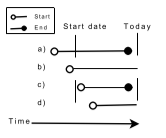
\includegraphics[width=0.5\linewidth]{gfx/slice.png}
\caption{Time slice and incomplete logs \nyi{redo}}
\label{fig:timeslice}
\end{figure}

% Incomplete traces in the chosen ''slice'' (events missing from beginning/end)
Second aspect to note is that when the event log data is used, the data being analyzed is always a "slice".
This means that it contains events from a time slice starting at some time instance $t_s$ and ending at some later time $t_e$. All events between these times are considered. A common use case would be to inspect the past 24 hours of events. In this case $t_e$ is the current time, and $t_s$ is the current time -24 hours. 
This results in the time slice containing a large amount of events that belong to a trace that started before $t_s$, or traces that have yet to be completed. This is illustrated in figure \ref{fig:timeslice}. These traces should be removed, since they appear to start from an event that is not a real starting point (respectively for the end). Classifying a trace as anomalous like this requires an \emph{appropriate model} \cite{bezerra2009anomaly}, 
i.e. some definition on how to find whether a trace is invalid.

% resubmissions
Another issue is splitting the traces form the event log, meaning identifying the individual cases.
For this specific system, each submission of a product in the system has an unique \emph{submission identifier} (submission ID).
This ID can be used to uniquely identify a trace. 
However, in the store systems the same application submission can be re-submitted.
This is commonly done if some part of the workflow fails.
The events in this re-submission cycle will have the same submission ID as the original submission.
This leads to a situation where the trace seems to restart from the beginning or from a different step and then finish. These cases should be identified as anomalous. In the case of real-time data, only the latest submission for each ID should be considered.

Another big challenge comes from the real-time characteristics of the data. Since all data describes the current state of the system, the underlying process model can change any time. Because of agile practices and continuous delivery, the store systems are under constant change. This means that the process model generated a day before may not reflect the current state anymore. The system should be flexible and should adapt to any changes in the underlying models.

% invalid states
Furthermore, the production data will include also traces that have failures or phases that are in progress.
A trace with failed or erroneous steps should be considered anomalous, since they are not guaranteed to progress normally after an error. 
Similarly, the traces include events that do not describe a final state, but only broadcast status. 
The most common type of event like this events with an ''In progress'' status.
If an event is non-final, it means that the same process is still expected to fire a final event afterwards.
These events should be handled differently in the modeling phase.

All these characteristics require that the system uses some kind of pre-processing method that takes the slice of the real-world data and outputs an ordered and grouped set of traces with the anomalous traces removed.

\subsection{Graph construction}

\subsubsection{Pre-processing}

To comply with the user requirements of being able to generate models from custom queries and real-time production data, the system developed in this thesis should be able to take any set of events as the input.
Because of the challenges outlined in the previous section, a pre-processing step is needed.

The pre-processing method chosen takes a set of events as the input. The pre-processing works as follows:
\begin{enumerate}
    \item Group all events by \textbf{submission ID}.
    \item Create a trace corresponding to a submission for each group.
    \item Order all events in each trace by ascending timestamp, then by event ID.
    \item Drop all traces with an erroneous event such as ''Failed''.
    \item Drop all non-final events from each trace.
\end{enumerate}
After these steps the result is a set of valid traces, each corresponding to a unique submission ID with only final events.

\subsubsection{Creating directed graphs}

The model chosen to represent the process models is the directed graph. 
In this model, every pair of directly subsequent events $(a,b)$ appearing in a trace corresponds to a 
graph edge from node $a$ to node $b$.
The parallelism is generated by observing the direct follow-relations as in the \textalpha-algorithm.

To generate a graph from a set of traces, I started by generating an event log \emph{footprint matrix}.
The footprint matrix describes the relation of all the events in the event log regarding to each other.
This means that the matrix describes which events immediately follow another events in the set of traces.
The columns and rows of the matrix correspond to all the distinct activities (the vocabulary).
The matrix is square and should have a zero diagonal.
The row describes the first event, and the column the event directly following.
The number in the cell describes the frequency that this follow relation was observed in the logs.

I will illustrate this with an example. Consider an event log with four activities $a,b,c,d,$ and $e$.
Figure \ref{fig:exampletraces} illustrates the six traces in the event log. There are two unique kinds of traces, $abcde$ and $acbde$, both of which have been observed three times. Figure \ref{fig:examplematrix} shows the footprint matrix generated from these traces.
The diagonal is zeroes, since no event follows itself.
From the upper triangle the matrix shows for example that $b$ has followed $a$ three times and $c$ has followed $b$ three times. From the lower triangle we see for example that $a$ has never followed $b$, but $b$ has followed $c$ three times.
By comparing the frequencies in the upper triangle to the lower triangle we can discover dependencies suggested by the event log, and from a lack of dependency we can suggest parallelism.

\begin{figure}
    \centering
    % example traces
    \begin{subfigure}[h]{0.4\linewidth}
        \begin{center}
        \begin{tabular}{| r | l |}
        Trace & Frequency \\
        \hline
        a b c d e & 3\\
        a c b d e & 3 \\
        \hline
        \end{tabular}
        \end{center}
        \caption{A list of example traces}
        \label{fig:exampletraces}
    \end{subfigure}
    % footprint example
    \begin{subfigure}[h]{0.4\linewidth}
        \begin{center}
        \begin{blockarray}{cccccc}
          & a & b & c & d & e\\
        \begin{block}{c(ccccc)}
        a & 0 & 3 & 3 & 0 & 0 \\
        b & 0 & 0 & 3 & 3 & 0 \\
        c & 0 & 3 & 0 & 3 & 0 \\
        d & 0 & 0 & 0 & 0 & 6 \\
        e & 0 & 0 & 0 & 0 & 0 \\
        \end{block}
        \end{blockarray}
        \end{center}
        \caption{An example footprint matrix $M$ }
        \label{fig:examplematrix}
    \end{subfigure}
    \caption{Example for traces containing events $\{a,b,c,d,e\}$}
\end{figure}

% turning the matrix into a graph
The generated footprint matrix corresponds directly to the log-based ordering relations described by van der Aalst and van Dongen \cite{van2013discovering,van2016process}.
There are four possible relations between any two events in an event log $L$:
\begin{itemize}
    \item $a \rightarrow_L b$: $b$ \emph{directly follows} $a$.
    \item $a \leftarrow_L b$: $b$ \emph{directly precedes} $a$.
    \item $a ||_L b$: $a$ and $b$ are \emph{parallel}.
    \item $a \#_L b$: $a$ and $b$ are not directly related, they are $unrelated$.
\end{itemize}

Note that it always applies that $a \rightarrow_L b \Leftrightarrow b \leftarrow_L a$.
We can find these relations from the footprint matrix by comparing each cell $m_{ij}$ the upper triangle with the corresponding cell $m_{ji}$ lower triangle by using the following algorithm:

\begin{definition}
Let $A = \{ a_i | 0 < i \le n \}$ be a set of $n$ activities (the \emph{vocabulary}).
Let $M$ be an $n \times n$ footprint matrix corresponding to $A$.
For each cell $m_{ij} \in M$ where $i < j$:
\begin{itemize}
    \item $a \#_L b$ iff $m_{ij} = 0$ and $m_{ji} = 0$
    \item $a_i \rightarrow_L a_j$ iff $m_{ij} > m_{ji}$ and $m_{ji} = 0$
    \item $a_i \leftarrow_L a_j$ iff $m_{ij} < m_{ji}$ and $m_{ij} = 0$
    \item $a_i ||_L a_j$ iff $m_{ij} > 0$ and $m_{ji} > 0$
\end{itemize}
Furthermore, it should be noted that these relations are symmetrical:
\begin{itemize}
    \item $a \#_L b \Leftrightarrow b \#_L a$ 
    \item $a_i \rightarrow_L a_j \Leftrightarrow a_j \leftarrow_L a_i$
    \item $a_i ||_L a_j \Leftrightarrow a_j ||_L a_i$ 
\end{itemize}
\label{def:logrelations}
\end{definition}

In the example, comparing the cell $M[a,b] = 3$ to cell $M[b,a] = 0$ we get $a \rightarrow b$. \nyi{formatting?}
However, by comparing $M[b,c] = 3$ to $M[c,b] = 3$ we see that $b || c$. 
Figure \ref{tab:examplefootprint} shows the generated footprint for the matrix shown in figure \ref{fig:examplematrix}.
Note that it is enough to only examine the upper triangle of the matrix, since the generated footprint is always symmetrical across the diagonal.

This footprint maps directly to a corresponding directed graph.
Every activity in the vocabulary corresponds to a graph node.
Every ''directly follows'' relation corresponds to a directed arc in the graph. A parallel relation corresponds to arcs in both directions.
Figure \ref{fig:examplegraph} shows the directed graph corresponding to the footprint from figure \ref{tab:examplefootprint}.


\begin{figure}
    \centering
    % example traces
    \begin{subfigure}[h]{0.4\linewidth}
        \begin{center}
        \begin{tabular}{cccccc}
        \hline
          & a & b & c & d & e\\
        \hline
        a & \# & $\rightarrow$ & $\rightarrow$ & \# & \# \\
        b & $\leftarrow$ & \# & || & $\rightarrow$ & \# \\
        c & $\leftarrow$ & || & \# & $\rightarrow$ & \# \\
        d & \# & $\leftarrow$ & $\leftarrow$ & \# & $\rightarrow$ \\
        e & \# & \# & \# & $\leftarrow$ & \# \\
        \hline
        \end{tabular}
        \end{center}
        \caption{Generated footprint}
        \label{tab:examplefootprint}
    \end{subfigure}
    % footprint example
    \begin{subfigure}[h]{0.4\linewidth}
        \centering 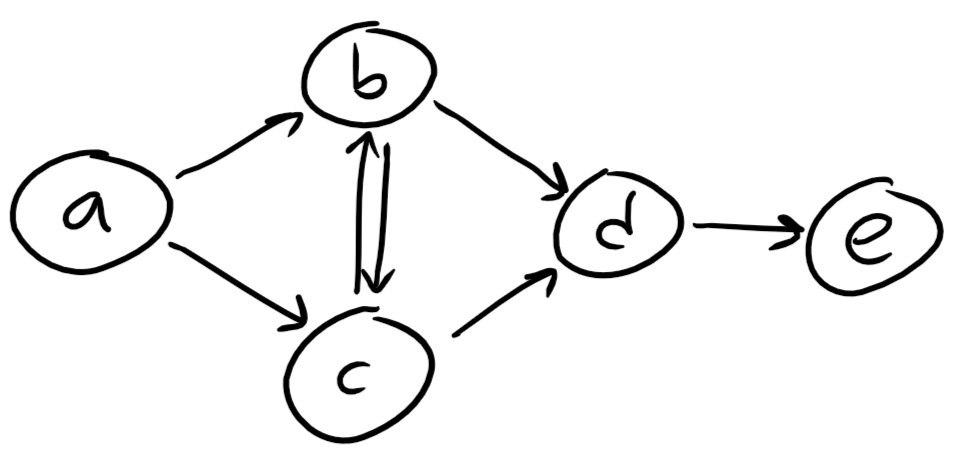
\includegraphics[width=\linewidth]{gfx/graphthing.jpg}
        \caption{Generated graph \nyi{remake}}
        \label{fig:examplegraph}
    \end{subfigure}
    \caption{Graph generation from the footprint}
\end{figure}

% Dealing with noise
Noise in the event log data creates problems if unhandled. 
\nyi{talk about noise}

\subsubsection{Statistics}

\nyi{Collecting statistics}\\
\nyi{Methods of generating median, TP75, TP90}\\
\nyi{What is different when using a predetermined JSON shape}

\subsection{Real-time functionality}

\nyi{Overlaying real-time data with generated process model}\\
\nyi{Generating a timeline view with start and end times from the overlay}\\
\nyi{Methods of finding the start times and dealing with parallelism}

\subsection{Estimating the future}

\nyi{Estimating future on incomplete logs}\\
\nyi{Statistical approach by using TP75}

\subsection{Machine learning}

\nyi{How ML approach could be used to improve the statistical approach}\\
\nyi{Explain models used (poisson \cite{azurepoisson}, bdt \cite{azurebdt} \cite{lambdamart2010})}\\
\nyi{Explain why these ones were chosen}

\nyi{Explain training dataset generation}

\nyi{Explain initial testing}\\
\nyi{Testing with noisy features removed (textual fields)}
\nyi{Explain additional features}\\
\nyi{ - identical resubmission}\\
%  posting that needed human interventiondcxfkkkkkkkkkkkkkkkkkkm
%                                       a cat did this ^ 
\nyi{ - posting that needed human intervention (manual review)}

\subsubsection{Azure ML}
\nyi{Explain briefly what azure ML is}

\subsection{Notifications}
\nyi{Describe how the estimates could be used for notifications}


%%%%%%%%%%%%%%%%%%%%%%%%%%%%%%%%%%%%%%%%%%%%%%%%%%%%%%%%%%%%%%%%%%%%%%%%%%%%%%%%
%%% Implementation
%%%%%%%%%%%%%%%%%%%%%%%%%%%%%%%%%%%%%%%%%%%%%%%%%%%%%%%%%%%%%%%%%%%%%%%%%%%%%%%%

\clearpage
\section{Implementation Details}

\nyi{Introduction}

\nyi{Explain integration with the existing system}

\nyi{SQL queries, C\# LINQ to SQL, combined with textual query}\\
\nyi{Talk about user-customized views}\\
\nyi{Everything based on user-made queries, even templates}\\

\nyi{Details about the simple footprint generation}\\
\nyi{Include tables/figures from observed noise to illustrate noise levels}\\

\nyi{Turning the footprint into a directed graph}

\nyi{Maybe: Talk about implementing the alternative graph? not much to say..}

\nyi{Implementing the option of reading the graph shape from a JSON definition file}

\nyi{Storing the graph, caching in DB, memory}

\nyi{Overlaying real-time data with the model}\\

\nyi{Estimate based on collected statistics}\\
\nyi{ - statistics}\\
\nyi{ - machine learning models}

\nyi{Constructing timeline from the graph}\\

\nyi{User Interface}\\
\nyi{vis js, asp.net mvc, etc}\\
\nyi{ - displaying the graph}\\
\nyi{ - merging of ''bubbles''}\\
\nyi{ - timeline view}\\
\nyi{ - multiple graphs/timelines per page}\\

\nyi{Make sure the difficulties are all mentioned somewhere}\\
\nyi{(you'll want these for the presentation)}\\
\nyi{ - parallelism}\\
\nyi{ - clock skew}\\
\nyi{ - changes in workflow}\\
\nyi{ - bugs manifesting in graphs (is this really a bad thing?)}\\
\nyi{ - dealing with rare events (manual review)}\\
\nyi{ - confidentiality}\\


%%%%%%%%%%%%%%%%%%%%%%%%%%%%%%%%%%%%%%%%%%%%%%%%%%%%%%%%%%%%%%%%%%%%%%%%%%%%%%%%
%%% Results
%%%%%%%%%%%%%%%%%%%%%%%%%%%%%%%%%%%%%%%%%%%%%%%%%%%%%%%%%%%%%%%%%%%%%%%%%%%%%%%%

\clearpage
\section{Results}
\label{sec:results}

%T\"ass\"a osassa esitet\"a\"an tulokset ja vastataan tutkielman alussa
%esitettyihin tutkimuskysymyksiin. Tieteellisen kirjoitelman
%arvo mitataan t\"ass\"a osassa esitettyjen tulosten perusteella.

\nyi{Graphs generated by the system (pictures!)}

\begin{figure}[htb]
\centering 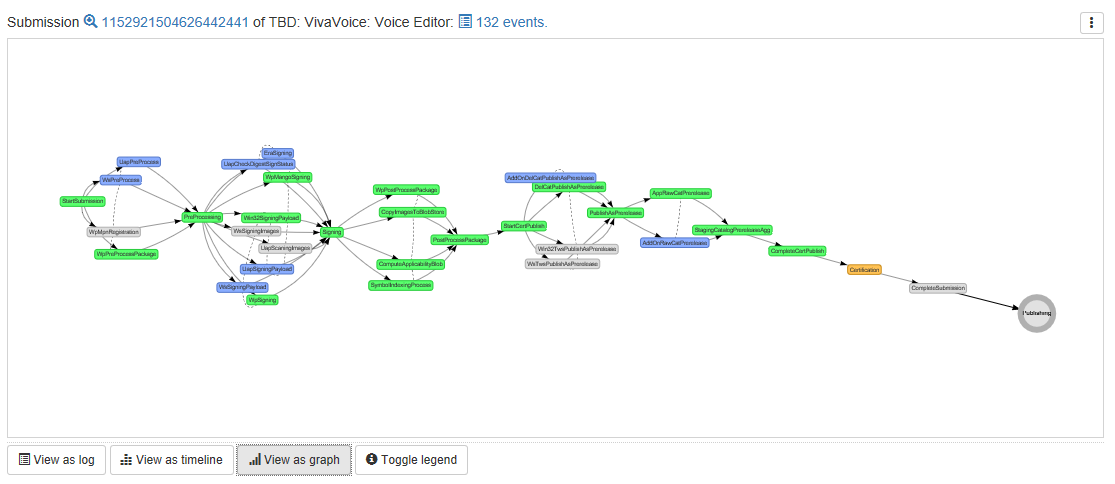
\includegraphics[width=\linewidth]{gfx/graph.png}
\caption{Graph view \label{fig:graph}}
\end{figure}

\begin{figure}[htb]
\centering 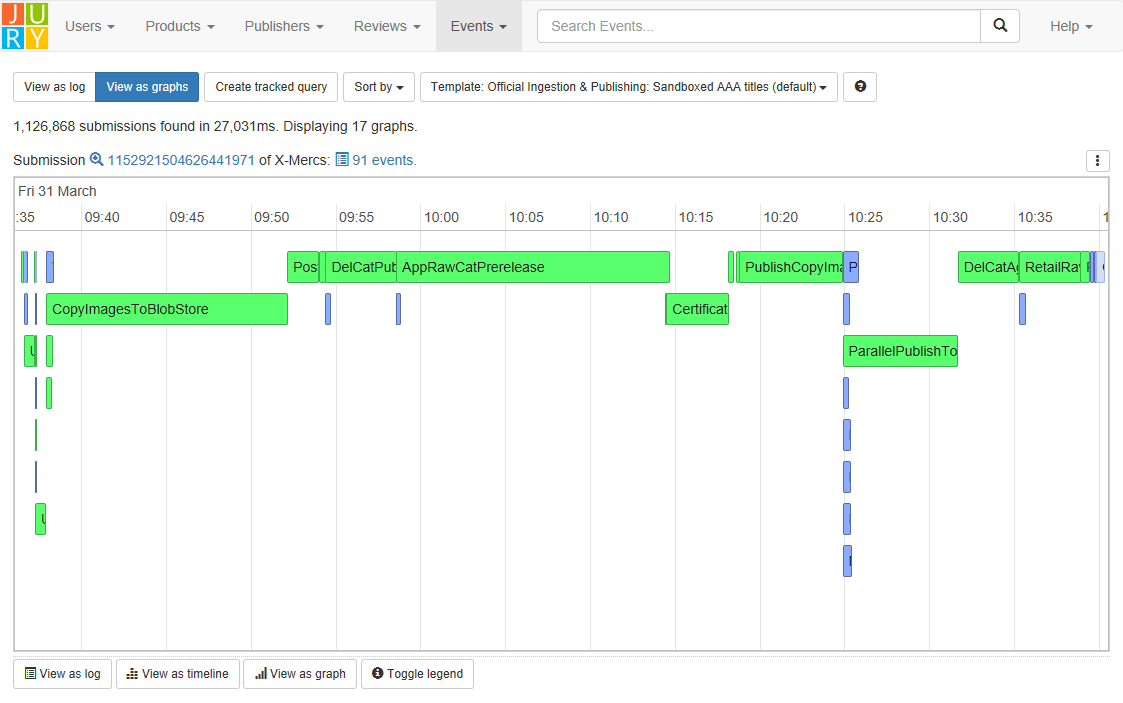
\includegraphics[width=\linewidth]{gfx/timeline.png}
\caption{Timeline view \label{fig:timeline}}
\end{figure}

\begin{figure}[htb]
\centering 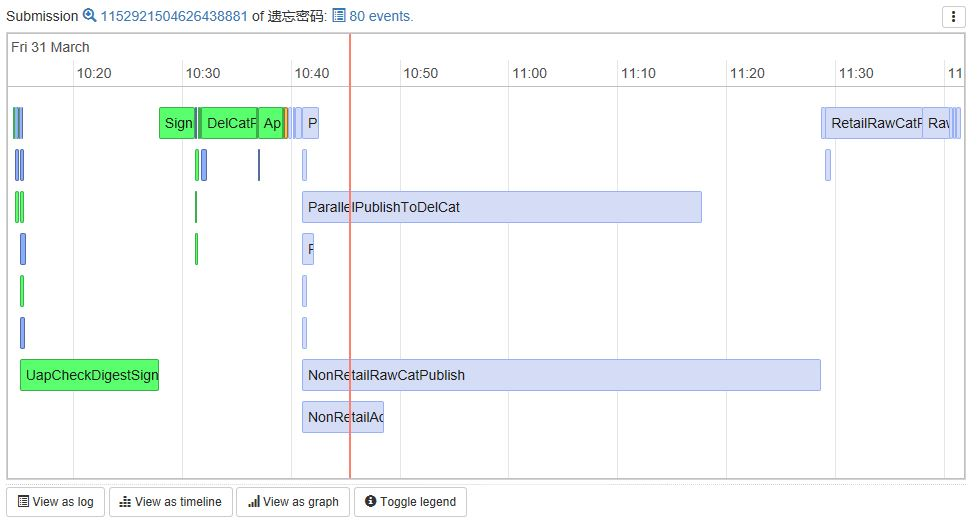
\includegraphics[width=\linewidth]{gfx/estimates.jpg}
\caption{Timeline view with estimates \label{fig:estimates}}
\end{figure}

\nyi{Statistics and their scores}
% (run stats on the same dataset)

\nyi{ML models and their scores}

\nyi{User satisfaction}

\subsection{Evaluation}
\label{sec:evaluation}

%Tutkimustuloksien merkityst\"a on aina syyt\"a arvioida ja tarkastella
%kriittisesti.  Joskus tarkastelu voi olla t\"ass\"a osassa, mutta se
%voidaan my\"os j\"att\"a\"a viimeiseen osaan, jolloin viimeisen osan nimeksi
%tulee >>Tarkastelu>>. Tutkimustulosten merkityst\"a voi arvioida my\"os
%>>Johtop\"a\"at\"okset>>-otsikon alla viimeisess\"a osassa. 

%T\"ass\"a osassa on syyt\"a my\"os arvioida tutkimustulosten luotettavuutta.
%Jos tutkimustulosten merkityst\"a arvioidaan >>Tarkastelu>>-osassa,
%voi luotettavuuden arviointi olla my\"os siell\"a. 

\nyi{Talk about success with graph generation}\\
\nyi{Maybe talk about alternative graph?}\\
\nyi{Changes in the system reflected real time (also a strength?)}\\
\nyi{Finding bugs in system (race conditions!) based on graphs}\\
\nyi{Feedback from users}

\nyi{Talk about negatives with machine learning models}\\
\nyi{Reason why they didn't end up working}

\nyi{Talk about how the system went immediately into production}\\
\nyi{Talk about the success of notifications built on top of the system}

%%%%%%%%%%%%%%%%%%%%%%%%%%%%%%%%%%%%%%%%%%%%%%%%%%%%%%%%%%%%%%%%%%%%%%%%%%%%%%%%
%%% Conclusions
%%%%%%%%%%%%%%%%%%%%%%%%%%%%%%%%%%%%%%%%%%%%%%%%%%%%%%%%%%%%%%%%%%%%%%%%%%%%%%%%

\clearpage
\section{Conclusions and Future Work} 
\label{sec:conclusions}

\begin{itemize}
\item[--]\nyi{Contributions (positives)}
\item[--]\nyi{Limitations (negatives)}
\item[--]\nyi{Future work}
\end{itemize}

%%%%%%%%%%%%%%%%%%%%%%%%%%%%%%%%%%%%%%%%%%%%%%%%%%%%%%%%%%%%%%%%%%%%%%%%%%%%%%%%
%%%%%%%%%%%%%%%%%%%%%%%%%%%%%%%%%%%%%%%%%%%%%%%%%%%%%%%%%%%%%%%%%%%%%%%%%%%%%%%%
%%% References
%%%%%%%%%%%%%%%%%%%%%%%%%%%%%%%%%%%%%%%%%%%%%%%%%%%%%%%%%%%%%%%%%%%%%%%%%%%%%%%%
%%%%%%%%%%%%%%%%%%%%%%%%%%%%%%%%%%%%%%%%%%%%%%%%%%%%%%%%%%%%%%%%%%%%%%%%%%%%%%%%

\clearpage
%% The \phantomsection command is necessary for hyperref to jump to the 
%% correct page, in other words it puts a hyper marker on the page.

\phantomsection
\addcontentsline{toc}{section}{References}

\printbibliography

%% Appendices
%\clearpage
%\thesisappendix

\end{document}
